% THIS DOCUMENT IS FOLLOWS THE VOLERE TEMPLATE BY Suzanne Robertson and James Robertson
% ONLY THE SECTION HEADINGS ARE PROVIDED
%
% Initial draft from https://github.com/Dieblich/volere
%
% Risks are removed because they are covered by the Hazard Analysis
\documentclass[12pt]{article}
\usepackage{graphicx}
\usepackage{booktabs}
\usepackage{tabularx}
\usepackage{hyperref}
\usepackage{float}
\usepackage{enumitem}
\usepackage{booktabs,tabularx,makecell}
\usepackage{caption}
\usepackage{xcolor,colortbl}
\captionsetup{font=small,labelfont=bf}
\newcolumntype{Y}{>{\raggedright\arraybackslash}X} 
\newcolumntype{Z}{>{\centering\arraybackslash}p{1.6cm}}
\hypersetup{
    bookmarks=true,         % show bookmarks bar?
      colorlinks=true,      % false: boxed links; true: colored links
    linkcolor=red,          % color of internal links (change box color with linkbordercolor)
    citecolor=green,        % color of links to bibliography
    filecolor=magenta,      % color of file links
    urlcolor=cyan           % color of external links
}
\usepackage{enumitem}
\newcommand{\lips}{\textit{Insert your content here.}}

%% Comments

\usepackage{color}

\newif\ifcomments\commentstrue %displays comments
%\newif\ifcomments\commentsfalse %so that comments do not display

\ifcomments
\newcommand{\authornote}[3]{\textcolor{#1}{[#3 ---#2]}}
\newcommand{\todo}[1]{\textcolor{red}{[TODO: #1]}}
\else
\newcommand{\authornote}[3]{}
\newcommand{\todo}[1]{}
\fi

\newcommand{\wss}[1]{\authornote{magenta}{SS}{#1}} 
\newcommand{\plt}[1]{\authornote{cyan}{TPLT}{#1}} %For explanation of the template
\newcommand{\an}[1]{\authornote{cyan}{Author}{#1}}

%% Common Parts

\newcommand{\progname}{SFWRENG 4G06 - Capstone Design Process}
\newcommand{\authname}{\textbf{Team 17, DomainX} \\
\\ Awurama Nyarko
\\ Haniye Hamidizadeh
\\ Fei Xie
\\ Ghena Hatoum             
}
\usepackage{hyperref}
    \hypersetup{colorlinks=true, linkcolor=blue, citecolor=blue, filecolor=blue,
                urlcolor=blue, unicode=false}
    \urlstyle{same}
                                


\begin{document}

\title{Software Requirements Specification for \progname: DomainX} 
\author{\authname}
\date{\today}
	
\maketitle

\pagenumbering{roman}
\begin{table}[hp]
\caption{Revision History} \label{TblRevisionHistory}
\begin{tabularx}{\textwidth}{llX}
\toprule
\textbf{Date} & \textbf{Developer(s)} & \textbf{Change}\\
\midrule
October 4, 2025 & Awurama Nyarko & Added Open Issues\\
October 4, 2025 & Awurama Nyarko & Added Off-the-Shelf Solutions\\
October 4, 2025 & Awurama Nyarko & Added New Problems\\
October 4, 2025 & Awurama Nyarko & Added Tasks\\
October 5, 2025 & Ghena Hatoum & Added Product Boundary \\
October 5, 2025 & Ghena Hatoum & Added Product Use Case Table \\
October 5, 2025 & Ghena Hatoum & Added Individual Product Use Cases (PUC's) \\
October 5, 2025 & Ghena Hatoum & Added Functional Requirements \\
October 5, 2025 & Ghena Hatoum & Added Look and Feel Requirements \\
October 5, 2025 & Ghena Hatoum & Added Usability and Performance Requirements \\
October 5, 2025 & Ghena Hatoum & Added Sections: Product Boundary to Usability and Performance Requirements\\
October 5, 2025 & Haniye Hamidizadeh & Added Sections: Operational and Environmental Requirements to Compliance Requirements\\
October 6, 2025 & Fei Xie & Added Sections: Cost to Ideas for Solution\\
October 6, 2025 & Fei Xie & First Draft of Sections: Cost to Ideas for Solution\\
October 8, 2025 & Fei Xie & Added Sections: Purpose of the Project to Naming Conventions and Terms\\
October 8, 2025 & Awurama Nyarko & Fixing Tables\\
\bottomrule
\end{tabularx}
\end{table}

~\newpage

\tableofcontents

~\newpage
\section{Purpose of the Project}
\subsection{User Business}
With the recent advancements in LLM, AI, and ML in general. There has been more interest in the ML area. Focusing on the Neural Network domain, it can feel like a wild west of software tools and packages available. Dealing with “bad” software can be frustrating, it can be hard to install, lacking in documentation, or being outdated. 
This can take precious times away from the actual research and development of the software the user wants, with the time spent on debugging the libraries used.
\\Following the “methodology to assess the state of best practice for Domain X” paper, we will apply the methodology to the Neural Network Library domain. 
To assist in the creation of this paper, we will also create a tool, whose main purpose is to simplify the process of gathering, visualizing and storing the data. This tool will than be reusable for future domains. 
\subsection{Goals of the Project}
The completion of this tool will make the data gathering process faster and more efficient for the current paper used to pilot the project. Future papers will than be able to use the tool to assist in their own data gathering for their domain.\\
We'll measure the success of the goals listed in the \href{https://github.com/thaafei/DomainX/blob/main/docs/ProblemStatementAndGoals/ProblemStatement.pdf}{Problem Statement and Goals} document by the research subteam's experience while using the tool. \\
A summary of the goals is provided below, for more information, please visit the above hyperlink.
\begin{enumerate}
  \item Interactive Data Table
  \item Automated Data Collection
  \item Automated Analytic Hierarchy Process (AHP)
  \item Data Visualization and Download
  \item Collaboration
\end{enumerate}
\section{Stakeholders}
The following includes stakeholders of our project, 
\subsection{Client}
\textbf{CAS Supervisor}: The CAS Supervisor is the main product owner of the tool. They are responsible for providing the main features requested, as well has having the final say in the presentation and features of the tool. When the tool is live, they will also have administrative access.
\\\\\textbf{Research Subteam}\label{research_subteam_client}: The research subteam will be actively using the tool. They are responsible for providing feedback to the product subteam on any pain points experienced while using the tool.
As well as accessing if the tool makes the current data gathering process easier, as compared to the previous ad-hoc method of using excel.
\subsection{Customer}
\textbf{Research Subteam/Future Students}: See \hyperref[research_subteam_client]{Research Subteam}.\\
\\\textbf{Future Students}\label{future_students}: Future students who interested in accessing the state of best practice for their specific domain. They have the same responsibilities as the Research Subteam.
\subsection{Other Stakeholders}
\textbf{Domain Expert}: The consultant for the research subteam during their work on the paper. This person has deep domain knowledge but won't necessarily know the technical software aspects of the domain.
\subsection{Hands-On Users of the Project}
\textbf{Research Subteam/Future Students}: See \hyperref[research_subteam_client]{Research Subteam}.\\\\
\textbf{Future Students}: See \hyperref[future_students]{Future Students}.\\\\
\textbf{Researchers/Industry Workers}: These are people who are interested in seeing the results of the research results for a domain. They are responsible for accessing the usability of the tool in the context of a read-only experience, and provide feedback to the product subteam.
\subsection{Personas}
\subsubsection{Kevin - Master's Student at McMaster University}
I’m Kevin, a master student at McMaster University currently working on the state of best practice for Domain X. I am extremely busy so I don’t want to spend too much time so i want to use a tool to decrease the amount of manual data inputting I need to do. I am adequately familiar with software, such as using the terminal and version control. However, my interests are more in the science aspect of computer science, so I don’t want to spent too long setting things up.
\subsubsection{Ashley - Research Scientist at X company}
I’m Ashley, a research scientist currently working in the ML/AI field. During my work, I need access to varies tools to assist me. I don’t want to create all the tools myself, preferring to use off-the-shelve, pre-existing libraries so I can focus on what actually matters. I’ve read through several tech blogs but they all rank the libraries differently, or don’t consider a big enough variety, and sometimes the libraries mentioned are outdated. I would like to have a consolidated source that can measure varying aspects of the library since as a researcher, I haven’t had as much experience with the DevOps process of the software lifecycle. I like to use packages and libraries that are easy to learn, install, and use.

\subsection{Priorities Assigned to Users}
\textbf{Key Users}:
\begin{itemize}
\item Research Subteam
\item Domain Expert
\end{itemize}
\textbf{Secondary Users}:
\begin{itemize}
\item CAS Supervisor
\item Researchers/Industry Workers
\end{itemize}

\subsection{User Participation}
\textbf{Research Subteam} \\
Actively using the tool during the writing of the paper. They should provide honest feedbacks on the experience when using the tool. Including any shortfalls, UI disagreements, and bugs.\\\\
\textbf{Domain Expert} \\
Has knowledge of the NN domain, will provide feedback on the research subteam’s list of libraries to access, as well as help verify the conclusions during the research process, to see if it is similar from what they have personally experienced. Estimated participation time of: 1-2 hours.
\\\\\textbf{CAS Supervisor} \\
During the user acceptance testing phase of the product. The CASE Supervisor should provide their honest feedback on their experience while using the tool, as they are the main administrator of the tool once it's live.

\subsection{Maintenance Users and Service Technicians}
\textbf{Project Maintainer} \\
The person responsible for updating the tool with new features, or fixing any existing bugs once the initial creators of the tool leaves. They were not present during the development of the tool, and will most likely be the future students who uses the tool for their domain research.
\\\\
\textbf{Infrastructure Team} \\
The infrastructure team at McMaster University will be responsible for hosting the project, and should ensure that the application is available for use and maintains data integrity of their database servers.
\section{Mandated Constraints}
\subsection{Solution Constraints}
\begin{itemize}
  \item Requirement: The product must be built utilizing existing McMaster University software and IT infrastructure.
  \item Rationale: This approach is mandated to avoid the client incurring costs associated with application and database hosting.
  \item Fit Criterion: Successful implementation depends on the necessary infrastructure components being formally approved and provided by McMaster University IT services.
\end{itemize}
\subsection{Implementation Environment of the Current System}
\begin{itemize}
  \item The current system relies on Excel spreadsheets that are saved and stored either on an individual's personal laptop (which has an unknown operating system) or in an online cloud storage environment.
\end{itemize}
\subsection{Partner or Collaborative Applications}
\begin{itemize}
  \item Excel integration is essential. Since Excel was the format utilized by the previous ad hoc tool, enabling planned import and export functionality will facilitate a smooth transition and allow for the potential backfilling of historical data.
\end{itemize}
\subsection{Off-the-Shelf Software}
N/A
\subsection{Anticipated Workplace Environment}
\begin{itemize}
  \item  The application must be fully functional on current and immediately previous stable versions of major web browsers (e.g., Chrome, Firefox, Safari, Edge).
\end{itemize}
\subsection{Schedule Constraints}
\begin{itemize}
  \item Tool must be built by April 6, 2026
  \item Research paper must be written and published by April 6, 2026
\end{itemize}
\subsection{Budget Constraints}
\begin{itemize}
  \item The project cannot cost more than \$125.
\end{itemize}
\subsection{Enterprise Constraints}
\begin{itemize}
  \item Project will be built using Microsoft related services.
\end{itemize}

\section{Naming Conventions and Terminology}
\subsection{Glossary of All Terms, Including Acronyms, Used by Stakeholders
involved in the Project}

The following terms and acronyms are used throughout this document and among project stakeholders.

\begin{description}[leftmargin=2.5cm, style=nextline]
  \item[NNL:] Neural Network Libraries.
  \item[ML:] Machine Learning.
  \item[AI:] Artificial Intelligence.
  \item[LLM:] Large Language Model.
  \item[CAS:] Computing and Software Department (McMaster University).
  \item[Methodology:] The structured process used to assess the state of best practice within a software domain.
  \item[Tool:] The software being developed to automate data collection, visualization, and storage.
  \item[Research Subteam:] The student group using the tool to apply the methodology and write the research paper.
  \item[Domain Expert:] An individual with specialized knowledge in neural networks who provides feedback and validation.
  \item[Supervisor:] The CAS faculty member overseeing the project.
  \item[State of Best Practice Paper:] The research paper summarizing findings from applying the methodology.
  \item[Infrastructure:] University-provided resources (hosting, databases, servers).
  \item[Excel Sheets:] Existing manual tools used for data collection.
  \item[Ad Hoc Method:] Informal, unstructured approach previously used for data gathering.
  \item[Stakeholders:] All individuals involved in or affected by the project (e.g., supervisor, researchers, domain expert).
\end{description}


\section{Relevant Facts And Assumptions}
\subsection{Relevant Facts}
The existing workflow relies on Excel sheets and bash scripts, which do not support automated data gathering.
\subsection{Business Rules}
Domain experts generally work Monday to Friday, 9 AM – 5 PM, and are unlikely to respond outside these hours.
\subsection{Assumptions}
McMaster University will provide the infrastructure required to host the application and make the necessary databases available for use.

\section{The Scope of the Work}
\subsection{The Current Situation}
Following the methodology listed:

\begin{enumerate}
    \item Domain is identified
    \item Research team gathers a preliminary list of packages fitting the domain
    \item Domain expert is consulted and helps determine if the packages fit the domain
    \item Data gathering commences for the finalized packages used
        \begin{enumerate}
            \item Optional: Interviewing or surveying industry users of the packages
        \end{enumerate}
    \item Research paper is written, with visuals generated from the data
\end{enumerate}

Current ways to consult the domain experts or industry users are done non-systematically, left to the discretion of the research team. The most common method is through email, but this can be difficult to track when multiple messages are sent or several people are being contacted simultaneously.

The data gathering process is performed using Excel spreadsheets, with each entry manually typed. This introduces inefficiencies and potential errors, motivating the need for an automated solution to streamline data collection, improve traceability, and reduce manual workload.

\subsection{The Context of the Work}
The Neural Network Libraries (NNL) Assessment Tool is a web-based application designed to automate the collection, evaluation, and visualization of data for comparing open-source deep learning libraries. It operationalizes an existing research methodology developed to assess the state of practice in software engineering, applying it specifically to neural network libraries (NNLs).

There is currently no automated system performing this type of assessment; existing workflows rely on manual data collection and Excel-based analyses. The tool introduces automation, consistency, and traceability across data gathering, scoring, and visualization activities.

The tool operates within McMaster University’s research environment and interacts with multiple adjacent systems for data input, authentication, hosting, and output management. These interactions define the boundaries and environment in which the tool functions.

\begin{figure}[H]
    \centering
    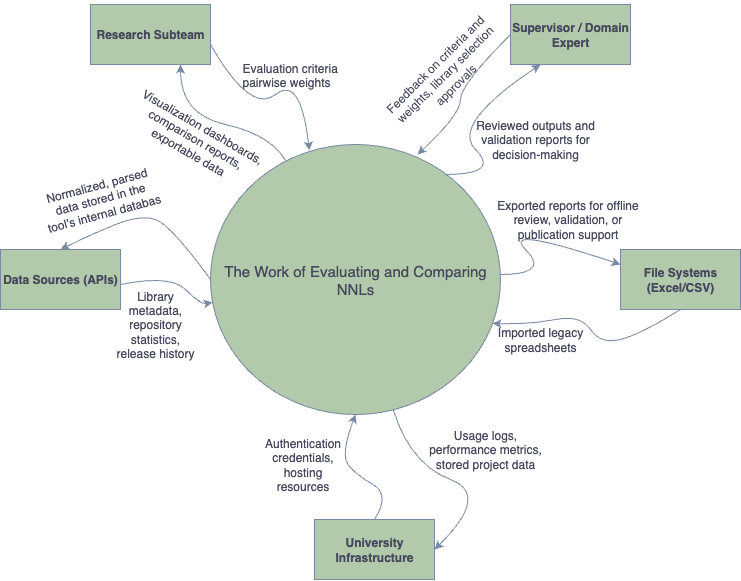
\includegraphics[width=\textwidth]{context-diagram.png}
    \caption{Work Context Diagram for the NNL Assessment Tool}
    \label{fig:context-diagram}
\end{figure}

\noindent
\textbf{Adjacent Systems:}
\begin{itemize}
    \item \textbf{Data Sources (APIs)} – GitHub, PyPI, and official library documentation, providing metadata, repository statistics, and release history.
    \item \textbf{Research Subteam} – Defines evaluation criteria and pairwise weights, initiates analyses, and reviews dashboards.
    \item \textbf{Supervisor / Domain Expert} – Reviews and validates library selections and output reports.
    \item \textbf{University Infrastructure} – Provides authentication services, hosting, and performance monitoring.
    \item \textbf{File Systems (Excel/CSV)} – Enables importing of legacy spreadsheets and exporting reports for offline review or publication.
\end{itemize}

\noindent
Each interface between the tool and adjacent systems represents an exchange of data or actions, as shown in Figure~\ref{fig:context-diagram}. Inputs include user-defined criteria and API data; outputs include processed datasets, analytical dashboards, and reports.

All data interfaces will align with the definitions in the Data Dictionary (Section~7).

\subsection{Work Partitioning}
\begin{table}[H]
\centering
\caption{Work Partitioning and Business Use Cases}
\begin{tabularx}{\textwidth}{|p{3.5cm}|X|X|}
\hline
\textbf{Event Name} & \textbf{Input \& Output} & \textbf{Summary of BUC} \\ \hline

New Library/Package Added for Assessment &
\textbf{Input:} Research subteam enters GitHub link or package name.  
\textbf{Output:} Tool retrieves metadata (stars, forks, releases, last commit) via API. &
System automatically fetches repository metrics from GitHub and stores them in the database for analysis and visualization. \\ \hline

Library Becomes Archived / Deleted / Restricted &
\textbf{Input:} API request fails or returns error.  
\textbf{Output:} Error log generated; library flagged for manual review. &
System detects inaccessible data and notifies research team to investigate and update records. \\ \hline

Domain Expert Revises Library List &
\textbf{Input:} Feedback from domain expert on selected packages.  
\textbf{Output:} Updated list of libraries for assessment. &
System allows easy modification of included libraries; re-runs analysis with updated list. \\ \hline

Assessment Cycle Completed &
\textbf{Input:} All data collected and validated.  
\textbf{Output:} Generated dashboards, ranking reports, and exportable visualizations. &
System computes AHP-based scores and produces comparative visualizations and reports for research publication. \\ \hline

\end{tabularx}
\end{table}

\subsection{Specifying a Business Use Case (BUC)}
Below is an example of a Business Use Case for a key event in the NNL Assessment Tool workflow.

\begin{table}[H]
\centering
\caption{Business Use Case Example – New Package Added to Domain}
\setlength{\tabcolsep}{4pt}
\renewcommand{\arraystretch}{1.2}
\footnotesize

\begin{tabularx}{\textwidth}{p{3cm} Y}
\toprule
\textbf{Business Event} & New library/package created for domain usage. \\
\midrule
\arrayrulecolor[gray]{0.8}
\textbf{Input(s)} & GitHub repository link and metadata retrieved from public API. \\
\hline
\textbf{Output(s)} & Stored library record in database; automated metrics collected (stars, forks, releases). \\
\hline
\textbf{Trigger} & Researcher adds new library or detects a new public repository. \\
\hline
\textbf{Primary Actor(s)} & Researcher. \\
\hline
\textbf{Secondary Actor(s)} & Domain Expert, System APIs. \\
\hline
\textbf{Preconditions} & API access is available; library URL is valid. \\
\hline
\textbf{Postconditions} & Library and metadata stored successfully; flagged for domain expert review. \\
\hline
\textbf{Main Flow} &
1. Researcher inputs new repository link. \newline
2. Tool fetches metadata from GitHub and related APIs. \newline
3. Data is validated and stored in the system database. \newline
4. Confirmation and logs generated. \\
\hline
\textbf{Alternative Flow(s)} &
– If API call fails, tool logs error and prompts user for manual data entry. \newline
– If duplicate record detected, tool alerts user and prevents duplication. \\
\hline
\textbf{Business Rules} &
– All repositories must belong to open-source libraries under the defined domain. \newline
– Collected metrics must be timestamped for version tracking. \\
\hline
\textbf{Exceptions} &
– API rate limits reached. \newline
– Network outage during data retrieval. \\
\bottomrule
\end{tabularx}
\end{table}


\section{Business Data Model and Data Dictionary}
\subsection{Business Data Model}
\begin{figure}[h!]
  \centering
  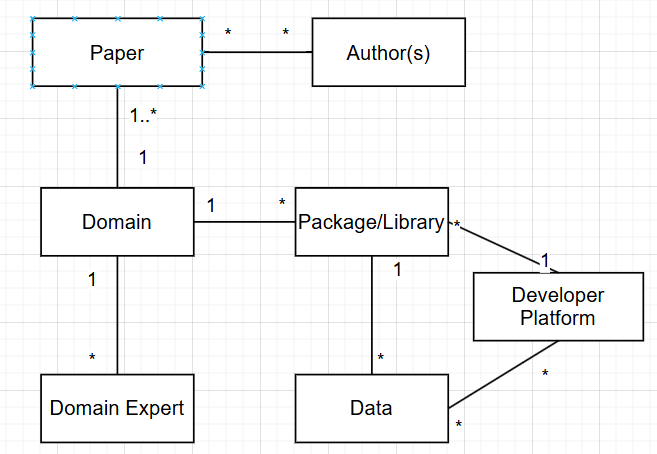
\includegraphics[width=0.8\textwidth]{BusinessDataModel.png}
  \caption{Business Data Model}
  \label{fig:business-data-model}
\end{figure}
\subsection{Data Dictionary}
\begin{table}[H]
\centering
\begin{tabularx}{\textwidth}{|l|X|l|}
\hline
\textbf{Name} & \textbf{Content} & \textbf{Type} \\ \hline
Paper & Paper Version + Paper Id + Paper Name & Class \\ \hline
Author/Contributor & Author Name, MacID & Class \\ \hline
Domain & Domain Name & Class \\ \hline
Packages/Library & Package Name + Github URL & Class \\ \hline
Data & Data description, Data Value & Class \\ \hline
Developer Platform & Package URL, Type, API Information & Class \\ \hline
Paper Version & \textit{See Paper} & Attribute/Element \\ \hline
Paper Id & \textit{See Paper} & Attribute/Element \\ \hline
Paper Name & \textit{See Paper} & Attribute/Element \\ \hline
Package Name & \textit{See Package} & Attribute/Element \\ \hline
Package URL & \textit{See Package} & Reference \\ \hline
Data Description & \textit{See Data} & Attribute/Element \\ \hline
Data Value & \textit{See Data} & Attribute/Element \\ \hline
Package URL & \textit{See Developer Platform} & Attribute/Element \\ \hline
Type & \textit{See Developer Platform} & Attribute/Element \\ \hline
API Information & \textit{See Developer Platform} & Attribute/Element \\ \hline
\end{tabularx}
\caption{Business Data Model Elements}
\end{table}


\section{The Scope of the Product}
\subsection{Product Boundary}
This system aims to simplify and streamline the process of collecting, managing, and analyzing data to assess the state of the practice for various research domains. It replaces the existing, manual process (currently managed via Excel sheets) and formalizes the methodology outlined in the \href{https://arxiv.org/abs/2110.11575}{Methodology for Assessing the State of the Practice for Domain X paper}. The final system will be a secure, accessible, data management and analysis tool.

The system will provide the following core functionality:
\begin{itemize}
  \item \textbf{Security and User Management:}
  \begin{itemize}
    \item Securely manage user accounts (login, password changes).
    \item Accounts can only be created by an administrator invitation.
    \item Enforce Role-Based Access Control (RBAC).
    \item Ensure only authenticated users can modify data.
  \end{itemize}
  \item \textbf{Data Integrity and Auditing:} Maintain an audit trail for all data entries, logging when a change is made.
  \item \textbf{Core Data Operations:} Facilitate the storing, updating, and retrieving of all core research entities: research domains, libraries, and collected metrics.
  \item \textbf{Data Collection:}
  \begin{itemize}
    \item Support mass data upload from previous research work.
    \item Automatically collect data to populate a specified data table (e.g., State-of-Practice Metrics Table).
  \end{itemize}
  \item \textbf{Analysis and Visualization:}
  \begin{itemize}
    \item Implement an AHP-based ranking of libraries within a domain based on their state of practice.
    \item Visualize data as different 2D graphs, showing the difference between libraries in a domain.
  \end{itemize}
  \item \textbf{User Experience (UX):}
  \begin{itemize}
    \item Have an intuitive UI to improve overall user experience.
    \item Ensure accessible read permissions for all users.
  \end{itemize}
  \item \textbf{Data Export:} Allow users to download tables or graphs onto their local device.
\end{itemize}

\noindent The following capabilities are explicitly excluded from the initial scope:

\begin{itemize}
  \item \textbf{Communication:} The system will not facilitate scheduling or hosting meetings between researchers and domain experts.
  \item \textbf{User Data:} Only username, email, and password will be collected for user profiles, no need for personal information.
  \item \textbf{Fine-Grained Permissions:} The system will not separate domain access by researcher. All authenticated researchers will be able to view and edit any domain.
  \item \textbf{Data/Library Recommendations:} The system will not give users suggestions on which library to use based on insufficient information.
  \item \textbf{Data Imputation/Handling:} The system will not automatically fill in missing data, nor will it incorporate a mechanism to assume the possibility of missing data during AHP calculation.
  \item \textbf{System Management:} The system will not include functionality for adding or removing administrator accounts.
  \item \textbf{AHP Validation:} The system will not include functionality to check the accuracy of the AHP calculations.
\end{itemize}

\noindent The following items are recognized as potential enhancements but are considered low-priority:

\begin{itemize}
  \item \textbf{Data Auditing:} Logging who edited the data entries.
  \item \textbf{Conflict Resolution:} Creating a method for merging changes when multiple users edit the same data simultaneously.
\end{itemize}

\subsection{Product Use Case Table}
\begin{tabularx}{\textwidth}{|p{2cm}|p{2cm}|p{2cm}|X|} \hline
\toprule
\textbf{Use Case (Goal)} & \textbf{Primary Actor} & \textbf{Secondary Actor(s)} & \textbf{Key Functional Requirements (FRs)} \\ \hline
\midrule
Invite New Users & Admin & Researcher & Admin can input a new user email. New user will receive an email with a link that will allow them to setup an account, password, and username. \\  \hline
Domain Creation \& Setup & Admin & Researcher & Create new Domain (must validate unique name). Optional: Add description to the domain. \\  \hline
Publish Domain & Researcher & General Users & Once the data collection is finished, allow anyone to see it (General Users). \\  \hline
Automation Library Data & Researcher & System & Auto-fill fields (e.g., creation date, commit date) upon entering a public URL. Check for and flag missing data that was expected to be collected. \\  \hline
Manually Input/Update Data & Researcher & System & Add missing data through the data table. Missing data must be highlighted in red. Only allow user to input right format (e.g., numbers, text). Maintain an audit trail of changes. \\  \hline
Ranking (AHP) & Researcher & System & System will run the integrated AHP tool using input quality scores and expert pairwise comparisons to automatically calculate the final package rankings. Run process automatically when the table is filled and updated. \\  \hline
Visualize \& Export Results & General User / Researcher / Admin & System & Allow selection of domain, libraries, and metrics to 2D graphs. Allow download of collected data (JSON/Excel). Allow download of graphs (PNG/LaTeX). \\  \hline
\bottomrule
\end{tabularx}

\subsection{Individual Product Use Cases (PUC's)}
Important things to keep in mind when looking at the at the Use Case Diagram:
\begin{itemize}
  \item Include: A  include B means, if A is executed that means B will be executed as well. 
  \begin{itemize}
    \item Update Data include Login, if user wanted to Update Data they must Login.
    \item Login include Verify Account, when user tries login the system will verify account.
  \end{itemize}
  \item Extend: A extends B means, if A is executed that means that B could be executed as well but not in all cases.
  \begin{itemize}
    \item Create New Domain extends Mass Data Upload:Create New Domain could also mean that the user wants to upload previous work, which would need a mass data upload, but not in all cases.
    \item Login extends Failed Login: When trying to login the user might fail to do so, however it's not always the case.
  \end{itemize}
\end{itemize}
\begin{figure}[H]
    \centering
    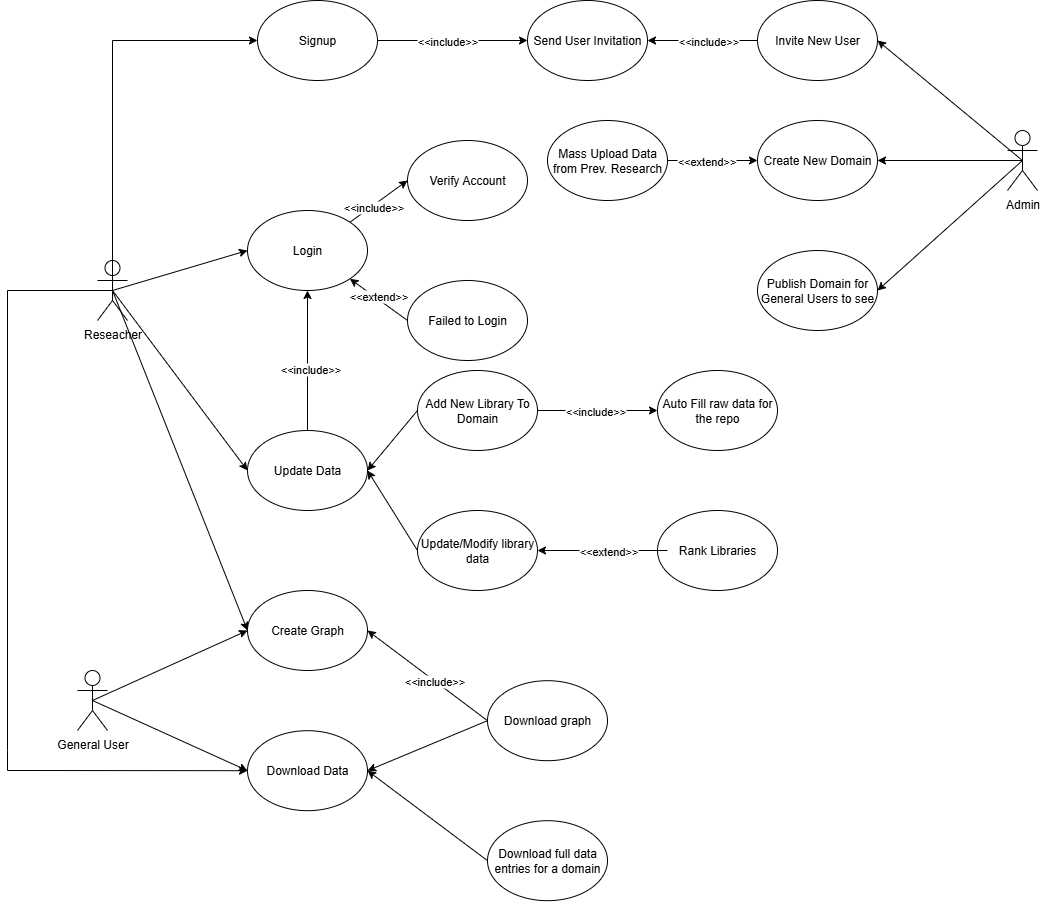
\includegraphics[scale=0.45] {usecase.png}
\end{figure}


\section{Functional Requirements}
\subsection{Functional Requirements}
\begin{enumerate}[label=FR\arabic*]
  \item The Admin will be able to extend an invitation to new researchers via the website, using the researcher's email address.
  \item Researchers will be able to sign up using their invited email. The process requires email validation and the creation of a unique username and password.
  \item The system will allow Admin and Researchers to securely log in using their email and password.
  \item Users will be able to reset their password after validating their email address.
  \item Admin can create domains, using a unique domain name and optionally a short description.
  \item Admin can publish a domain, once research is completed, for anyone to see and download data collected.
  \item Researchers can add/modify data/libraries of existing domains, and download data/graphs regardless of completion status.
  \item The system must validate all user input upon addition or update (e.g., ensuring numeric fields are numbers, dates are valid, and text limits are met).	
  \item The system must allow a Admin to bulk upload library and metric data using a predefined Excel template. The system must report detailed errors for any records that fail validation, such as feature names not being in the scope or wrong data type for a column.
  \item When a Researcher enters a public GitHub URL for a library, the system must call the GitHub API to automatically retrieve and populate specific data points, such as the Repository Creation Date and the Last Commit Date.
  \item The system must display a complete list of all metrics and their definitions for a selected domain.
  \item The system will rank the libraries within a domain using the Analytical Hierarchy Process (AHP) and display the calculated results.
  \item Users must be able to select a domain → libraries → metrics → graph type to visualize differences in libraries using comparative graphs.
  \item All users will be able to download the collected data for a specific scope in JSON, Excel, or LaTeX code formats to their device.
  \item Users must be able to download any generated graph, with the option to save it as a PNG file.
\end{enumerate}

\section{Look and Feel Requirements}
\subsection{Appearance Requirements}
\begin{enumerate}[label=LF-AR\arabic*]
  \item The application will maintain a consistent visual hierarchy where primary action buttons (e.g., "Save," "Create New Domain") are visually distinct.
  \item The system must be fully responsive and function correctly on standard desktop monitors and laptops.
  \item Data visualization and editing displays must prioritize information density while remaining readable. Tables should have alternating row colors (zebra striping) to help tracking.
  \item The main user dashboard should provide a clear, high-level overview of active domains and tasks, with minimal visual clutter.
  \item Ensure all required input fields are clearly identified (e.g., with an asterisk). Input forms must give real-time feedback, such as a green check mark for acceptable input and a red boundary for errors.
  \item All error messages (system errors, validation problems) must be clear, short, and contain practical guidance for resolving the problem.
\end{enumerate}
\subsection{Style Requirements}
\begin{enumerate}[label=LF-SR\arabic*]
  \item The system must use a single, consistent style of icons (e.g., solid, outline, or filled) for all navigational elements, actions, and status indicators.
  \item Graphs must use minimalist design to prioritize data readability. Axes and labels must be clear and legible.
  \item Font sizing must follow a defined scale (e.g., large for titles, medium for body text, small for captions) and remain consistent on all screens.
\end{enumerate}

\section{Usability and Humanity Requirements}
\subsection{Ease of Use Requirements}
\begin{enumerate}[label=UH-EU\arabic*]
  \item The primary navigational structure should be clearly defined and constantly available, with no prior training required for basic data viewing and download.
  \item Each library metric must have help icon that would tell the user what data type would be accepted.
  \item All errors will give clear and concise explanation.
\end{enumerate}
\subsection{Personalization and Internationalization Requirements}
N/A
\subsection{Learning Requirements}
\begin{enumerate}[label=UH-LR\arabic*]
  \item The system must contain a brief lesson or guide that explains the precise steps for Bulk Data Upload and the AHP Ranking process and is available from the appropriate screens.
  \item All words referring to research entities (Domain, Library, Metric) must be used consistently across the interface and documentation.
\end{enumerate}
\subsection{Understandability and Politeness Requirements}
\begin{enumerate}[label=UH-UP\arabic*]
  \item The system must contain a brief lesson or guide that explains the precise steps for Bulk Data Upload and the AHP Ranking process and is available from the appropriate screens.
  \item All words referring to research entities (Domain, Library, Metric) must be used consistently across the interface and documentation.
  \item All system-generated error messages will be clear, use non-technical language, and suggest a simple course of corrective action
\end{enumerate}
\subsection{Accessibility Requirements}
\begin{enumerate}[label=UH-AR\arabic*]
  \item Critical status indicators and data visualizations must convey meaning through patterns or text labels in addition to color.
  \item Users must be able to change font size using regular browser options (up to 200\%) without losing information or functionality.
\end{enumerate}

\section{Performance Requirements}
\subsection{Speed and Latency Requirements}
\begin{enumerate}[label=PR-SL\arabic*]
  \item All key data viewing and dashboard pages must load completely and become interactive within 3 seconds.
  \item The system must finish the AHP ranking calculation for a standard domain in less than ten seconds.
\end{enumerate}
\subsection{Safety-Critical Requirements}
\begin{enumerate}[label=PR-SC\arabic*]
  \item The system will encrypt all user passwords.
  \item If there have been multiple failed attempts to login to an existing account the user must be notified and lock account.
  \item The system will ensure that only researchers modify data.
\end{enumerate}\subsection{Precision or Accuracy Requirements}
\begin{enumerate}[label=PR-PA\arabic*]
  \item All data  that the system automatically filled out, must be 100\% accurate.
\end{enumerate}
\subsection{Robustness or Fault-Tolerance Requirements}
\begin{enumerate}[label=PR-RFT\arabic*]
  \item The system must implement graceful error handling, ensuring that a failure in one function (e.g., a failed GitHub API call) does not crash the entire application or disrupt other users.
  \item The system must use database transactions to ensure that data modifications are atomic, if an update operation fails in the middle, the data must be returned to its last validated state.
\end{enumerate}
\subsection{Capacity Requirements}
\begin{enumerate}[label=PR-CR\arabic*]
  \item The system must be able to accommodate up to 20 concurrent active users (logged in and doing operations) with no visible performance decrease.
  \item The database must be constructed to accommodate at least 10 different study domains.
\end{enumerate}
\subsection{Scalability or Extensibility Requirements}
\begin{enumerate}[label=PR-SE\arabic*]
  \item The system architecture must clearly divide the Data Management/Storage layer from the Analysis/Visualization layer so that either component may be improved or replaced independently.
  \item The authentication and authorization system must be adaptable enough to accommodate additional user roles (e.g., "Guest Analyst") and specialized rights without requiring code changes to core operations.
\end{enumerate}
\subsection{Longevity Requirements}
\begin{enumerate}[label=PR-LR\arabic*]
  \item The system must be capable of running without the requirement for maintenance for two years. 
\end{enumerate}

\section{Operational and Environmental Requirements}
\subsection{Expected Physical Environment}

\begin{enumerate}[label=OE-EPE\arabic*]
\item The tool is a web-based application that will be used mainly by our team, supervisors, and potentially other researchers or domain experts.
\item It is expected to run on a standard desktop or laptop computer with a reliable internet connection, in a normal indoor setting such as an office, lab, or home workspace.
\item No specialized hardware or rugged equipment is required. A keyboard, mouse, or touchpad, and a modern web browser (e.g., Chrome, Firefox, Edge) are sufficient.
\end{enumerate}

\subsection{Wider Environment Requirements}
\begin{enumerate}[label=OE-WE\arabic*]
\item The application depends on a stable internet connection for retrieving data from public repositories (e.g., GitHub) and for loading the hosted web interface if deployed to the cloud.
\item It does not rely on any dedicated on-premises hardware.
\item The tool should work on the latest two to three major versions of common browsers such as Chrome, Firefox, and Edge. No special environmental conditions (lighting, noise, temperature) are expected to affect usability.
\end{enumerate}
\subsection{Requirements for Interfacing with Adjacent Systems}
The tool must be able to communicate with a few external systems and internal components to collect, store, and visualize data.

\begin{enumerate}[label=OE-IA\arabic*]

  \item Public Repository APIs (e.g., GitHub API): The tool must communicate with external repository services to automatically collect information about the selected neural-network libraries. For example, it needs to retrieve details such as how often the code is updated, the number of open or closed issues and pull requests, and the main programming languages used. This data will help evaluate qualities like maintainability, transparency, and overall project activity. The information must be received in a standard machine-readable format (e.g., JSON over HTTPS) whenever a user triggers a scan or during scheduled updates.

  \item Database (MySQL): The backend must store scores, rankings, and evidence collected from repositories.

  \item Visualization Component: The frontend must render charts and comparisons (e.g., using Chart.js) from the data served by the backend.

  \item All connections must use standard web technologies (HTTP/HTTPS, JSON) and require only basic authentication methods such as API tokens for secure access to external repository APIs.

\end{enumerate}

\subsection{Productization Requirements}
The tool will be delivered as an open-source web application hosted in the team’s public GitHub repository.
\begin{enumerate}[label=OE-PR\arabic*]
\item A clear README file must explain how to set up the backend (Python + Flask) and the frontend (React) using common package managers such as pip and npm.
\item For developers running the tool locally, the repository must include a requirements.txt file for Python packages and a database schema file so they can create the required tables.
\item When deployed on a cloud platform such as AWS or Google Cloud, users must be able to access the tool directly through a web URL without installing anything.
\item The application must also provide options to export results in formats such as CSV for data tables and PNG/PDF for visualizations.
\end{enumerate}
\subsection{Release Requirements}
\begin{enumerate}[label=OE-RR\arabic*]
\item The project should follow the official capstone timeline: an internal test release before the Proof-of-Concept (PoC) demonstration in \textbf{November}, a Revision~0 Demonstration in \textbf{Weeks~18--19}, and the Final Release (Revision~1) at \textbf{Week~26} along with the research paper and final dataset.
\item The Final Release (Revision 1) must incorporate feedback collected during the Revision 0 Demonstration, including usability improvements, bug fixes, and supervisor/TA-requested changes.
\item All releases must be published as GitHub Releases and include a short changelog describing the changes in each version.

  \item Releases must use a clear, descriptive version tag such as the \texttt{MAJOR.MINOR.PATCH} format (or an equally descriptive format):
    \begin{itemize}
        \item \textbf{MAJOR:} Increased only when a change breaks backward compatibility (e.g., a database schema change that makes older data unusable).
        \item \textbf{MINOR:} Increased when adding new features that remain fully compatible with previous versions.
        \item \textbf{PATCH:} Increased for bug fixes or small improvements that do not affect existing features.
    \end{itemize}

  Example version tags:
    \begin{itemize}
        \item \texttt{v0.1.0} → first working prototype for the Revision~0 Demonstration
        \item \texttt{v0.2.0} → adds a new feature such as exporting the table to a CSV file
        \item \texttt{v0.2.1} → fixes a small bug in the export feature (patch)
        \item \texttt{v1.0.0} → stable Final Release for Revision~1
    \end{itemize}
\end{enumerate}
\section{Maintainability and Support Requirements}
\subsection{Maintenance Requirements}
The tool is an open-source web application that will need occasional updates to fix bugs and to adapt if external APIs change.
\begin{enumerate}[label=MS-MR\arabic*]
\item All code must follow the project’s coding standards (PEP 8 for the Python backend; React + TypeScript style guide for the frontend).
\item Automated tools (such as Black, Flake8, and Pylint) must remain part of the workflow so new contributors can easily read and update the code.
\item Unit tests must be written for all new features and bug fixes. Developers should also run basic integration tests to make sure the full pipeline (API → database → visualization) still works after changes.
\item Test coverage must be tracked and reported to ensure that critical parts of the backend are being tested.
\item All Python and frontend packages must be listed in requirements.txt and package.json, with pinned versions so the same build can be reproduced.
\item The dependency list must be reviewed and updated at least once each semester to keep it current and secure.
\item Any changes to the dataset made through the interactive data table must be logged with a timestamp and the username so there is always a clear audit trail.
\item Most routine fixes, such as small UI tweaks or bug fixes, should be finished within a couple of days. Larger updates, such as adding a new metric or a new visualization, are expected to take about one to two weeks.
\end{enumerate}
\subsection{Supportability Requirements}
The tool is intended to be mostly self-supporting since it will be used primarily by our team, the supervisors, and potentially other researchers in the future.
\begin{enumerate}[label=MS-SR\arabic*]
\item The README file must include step-by-step instructions so that a new developer can set up the backend (Flask + MySQL) and frontend (React) locally, or deploy it to a cloud platform (such as AWS or Google Cloud), in a consistent and repeatable way. A new developer should be able to follow these instructions and have the application running within about two hours.
\item The repository must always include an up-to-date guide for installation, setup, the data-collection workflow, using the interactive data table, visualization, and exporting results.
\item The backend must include logging to record API failures (such as rate-limit errors or unexpected data formats), database issues, and runtime exceptions so that maintainers can troubleshoot problems quickly.
\item Users should use the GitHub Issues page to report bugs or ask questions. No printed manual will be needed; all documentation will remain online in the repository.
\end{enumerate}
\subsection{Adaptability Requirements}
\begin{enumerate}[label=MS-AR\arabic*]
\item The tool must remain flexible so it can grow with the project and adapt to future needs.
\item The MySQL database must be set up so that if a new quality criterion needs to be tracked, it can be added by creating a new column, updating the data-collection script, and adjusting the UI without having to redesign the whole system.
\item The data-collection module must allow new data sources (for example, another code-hosting site or a different metrics service) to be added with minimal extra code and without disrupting the existing GitHub integration.
\item The tool must be able to run on standard operating systems(Windows, macOS, and Linux) by using widely supported technologies (such as Python, Node.js, and MySQL), and by avoiding any system-specific code.
\item The system must be designed in a modular way so that parts like data collection, storage, and visualization remain separate. This makes it easier to add new features or update one part without affecting the rest of the tool.
\end{enumerate}
\section{Security Requirements}
\subsection{Access Requirements}


\begin{enumerate}[label=SR-AC\arabic*]

  \item The tool must be open for anyone to view results, but only approved team members or domain experts may modify the data.

  \item The system must support two user roles:
    \begin{itemize}
        \item \textbf{Viewer:} Can view all interactive data tables that list the libraries, their scores, and rankings, along with all visualizations.
        \item \textbf{Contributor:} Has all Viewer permissions plus the ability to edit data in the interactive table.
    \end{itemize}

  \item Editing or any other administrative actions must be available only to logged-in users with the \textbf{Contributor} role.

  \item User roles (Viewer / Contributor) must be assigned and updated correctly at sign-up or by an admin so that permissions always reflect the intended access level.

  \item The system must display clear error messages for login failures (e.g., invalid credentials, network errors) and provide a secure way for users to recover or reset their account credentials.

  \item API credentials such as keys or tokens for external services (e.g., repository APIs) must be stored securely outside the source code (e.g., in environment variables) and must never be exposed in the frontend or version control.

\end{enumerate}

\subsection{Integrity Requirements}
\begin{enumerate}[label=SR-INT\arabic*]
\item To ensure the accuracy and reliability of the collected data, all manually entered information into the interactive table must be checked before it is saved. For example, numbers must fall within valid ranges, and text must be cleaned so that it cannot be treated as code or scripts.
\item The database must include safeguards so that if two users edit the same record at the same time, no changes are lost or overwritten.
\item The system must detect simultaneous edits and either block one save or notify the users to resolve the conflict.
\item When automated data updates conflict with a user’s manual edits (if any are updated automatically), the system must warn the user or request confirmation before replacing existing data.
\item The system must also store the raw evidence, calculated scores, and final rankings in separate fields so that the original data and results cannot be accidentally modified.
\item Publishing visualizations must not occur at the same time as data edits or automated refreshes. The system must either block publishing or enforce downtime until updates are complete.
\item If an export (e.g., CSV, PNG) fails or produces a corrupted file, the tool must alert the user and allow them to retry the download.
\end{enumerate}
\subsection{Privacy Requirements}
The tool mainly works with open-source repository data, so there is very little personal data involved.
\begin{enumerate}[label=SR-P\arabic*]
\item If basic user details are collected for login (such as name or email), they must be kept private and stored securely using widely accepted security standards.
\item User passwords must be stored only in hashed form using a secure one-way hashing algorithm so that the actual password is never saved.
\end{enumerate}
No other personal or confidential information will be collected or stored.
\subsection{Audit Requirements}
\begin{enumerate}[label=SR-AU\arabic*]
\item The system must keep a record of all important activity for accountability and troubleshooting. Every time a Contributor adds, edits, or deletes data in the interactive table, the system must save a log entry showing the user’s ID, the time of the action, the type of action, and the fields that were changed.
\item The system must also log key events such as login attempts (successful and failed), scheduled API-collection runs, and major errors so that they can be reviewed later.
\item Access to these logs must be restricted to authorized project admins only.
\end{enumerate}
\subsection{Immunity Requirements}
\begin{enumerate}[label=SR-IM\arabic*]
\item The backend must prevent SQL-injection attacks by using the safe query methods provided by the database library instead of building raw SQL strings with user input.
\item The frontend must display any text entered by users as plain text only and never allow it to run as code. For example, React’s built-in escaping already takes care of this.
\item The automated data-collection scripts must respect the rate limits of external repository APIs (e.g., GitHub). If a limit is reached, the scripts should pause and retry later rather than keep sending requests and risk overloading the service.
\item All Python and React libraries must be kept up to date, so the project does not rely on outdated packages with known security issues. There should also be a tool in place to regularly check for known vulnerabilities in these libraries, such as GitHub Dependabot.
\end{enumerate}

\section{Cultural Requirements}
\subsection{Cultural Requirements}
Since the tool will be shared mostly in an academic and research setting, we just need to make sure the interface stays clear, neutral, and easy to understand for anyone who uses it later.
\begin{enumerate}[label=CU-CR\arabic*]
\item \textbf{Language:} All text in the user interface and documentation must be in plain English. We should avoid using region-specific jargon so that future collaborators from outside McMaster can understand it easily.
\item \textbf{Dates and Numbers:} Dates must be displayed in a clear standard format such as ISO 8601 (YYYY-MM-DD) so they’re unambiguous for anyone who uses the tool. Numbers must use a consistent style (for example, decimal point for fractions and thousands separated by commas).
\item \textbf{Neutral Design:} Colours, labels, and icons must stay neutral and must not include any symbols or words that could carry unintended cultural or political meaning.
\item \textbf{Open-Source Norms:} The repository must include a license notice and simple contribution guidelines to match common open-source practice.
\end{enumerate}
\section{Compliance Requirements}
\subsection{Legal Requirements}
\begin{enumerate}[label=CR-LR\arabic*]
\item The tool must include a copyright notice covering the code and documentation produced by the team.
\item It must be distributed under an appropriate open-source license so that others can reuse it under clearly defined terms.
\item Users of the tool or any data generated by it are required to provide proper citation or acknowledgement when they use it in their own work.
\end{enumerate}
\subsection{Standards Compliance Requirements}
\begin{enumerate}[label=CR-STD\arabic*]
\item N/A
\end{enumerate}

\section{Open Issues}

Below is a list of factors and questions that remain unresolved and could significantly influence the design, functionality, or deployment of the Neural Network Libraries (NNL) Assessment Tool.

The purpose of identifying these open issues is to ensure they are tracked, managed, and resolved in a timely manner. Maintaining visibility of these uncertainties supports effective risk management and informed decision-making throughout the development lifecycle.

\subsection{List of Open Issues}
\begin{table}[H]
\centering
\caption{Open Issues to Track and Resolve}
\setlength{\tabcolsep}{5pt}
\renewcommand{\arraystretch}{1.2}
\footnotesize

\begin{tabularx}{\textwidth}{Z Y Y Y Y Z}
\toprule
\makecell{\textbf{Issue}\\\textbf{\#}} &
\textbf{Summary} &
\textbf{Cross-Reference} &
\textbf{Stakeholders Involved} &
\textbf{Action Required} &
\textbf{Status} \\
\midrule
\arrayrulecolor[gray]{0.8}

OI-01 & Finalization of hosting environment (e.g., internal server) & Section 13 -- Operational Requirements & CAS Supervisor, Infra Team & Confirm approved infrastructure with McMaster IT & Pending \\
\hline
OI-02 & Confirmation of the final list of Neural Network Libraries & Section 6 -- Scope of Work & Research Subteam, Domain Expert & Schedule review meeting with domain expert & Pending \\
\hline
OI-03 & Selection of UI framework and visualization library & Section 9 -- Functional Requirements & Development Team & Evaluate and finalize tech stack & In Progress \\
\hline
OI-04 & Clarification of Excel integration level (import/export vs live sync) & Section 9 -- Functional Requirements & Research Subteam, Developers & Define required use cases and confirm feasibility & Pending \\
\hline
OI-05 & Decision on authentication method (SSO vs custom login) & Section 9 -- Functional Requirements & CAS Supervisor, Development Team & Meet with IT to assess SSO feasibility & Pending \\
\hline
OI-06 & Confirmation of data storage architecture (SQL vs cloud) & Section 13 -- Operational Requirements & Developers, Infra Team & Evaluate hosting options and finalize design & Pending \\
\bottomrule
\end{tabularx}
\end{table}





\section{Off-the-Shelf Solutions}

This section identifies existing tools, software, and components that could be leveraged to reduce development time and cost for the Neural Network Libraries (NNL) Assessment Tool. It outlines reusable libraries and products that can be legally copied or adapted to accelerate development and ensure maintainability.

The goal is to reuse proven, reliable components and avoid reinventing existing functionality, thereby optimizing development effort and leveraging established best practices.

\subsection{Ready-Made Products}

Several existing platforms provide partial functionality aligned with the tool’s goals, particularly in data visualization, analytics, and automation. However, none fully satisfy the requirement for automated data gathering, Analytic Hierarchy Process (AHP) analysis, and integrated visualization.

\begin{table}[H]
\centering
\caption{Ready-Made Products Relevant to the NNL Assessment Tool}
\setlength{\tabcolsep}{4pt}
\renewcommand{\arraystretch}{1.2}
\footnotesize

\begin{tabularx}{\textwidth}{p{3cm} Y Y Y}
\toprule
\textbf{Product} & \textbf{Description} & \textbf{Relevance to Project} & \textbf{Limitations} \\
\midrule
Microsoft Excel &
Spreadsheet with storage, formulas, and charts. &
Used as baseline for current manual process. &
Lacks automation, scalability, and centralized access. \\
\arrayrulecolor[gray]{0.8}\hline
Google Sheets &
Cloud-based collaborative spreadsheet. &
Enables multi-user editing and sharing. &
Limited automation; manual data import. \\
\hline
Power BI / Tableau &
Advanced analytics and visualization tools. &
Suitable for dashboards and comparative graphs. &
Licensing cost; limited AHP customization. \\
\hline
SurveyMonkey / Google Forms &
Online data collection tools. &
Useful for gathering expert feedback. &
No direct database or analytics integration. \\
\bottomrule
\end{tabularx}
\end{table}



These products may serve as inspiration or integration points (e.g., Excel import/export) but cannot replace the custom automation and analysis required by the NNL Assessment Tool.

\subsection{Reusable Components}

The following open-source libraries and frameworks will be incorporated to support data collection, analysis, and visualization.

\begin{table}[H]
\centering
\caption{Reusable Components}
\setlength{\tabcolsep}{4pt}
\renewcommand{\arraystretch}{1.2}
\footnotesize

\begin{tabularx}{\textwidth}{p{2.7cm} Y Y Y}
\toprule
\textbf{Component} & \textbf{Purpose} & \textbf{Source} & \textbf{Justification} \\
\midrule
\arrayrulecolor[gray]{0.8}
Python Pandas &
Data manipulation and analysis. &
Open-source &
Handles tabular data and transformations efficiently. \\
\hline
Requests (Python) &
Retrieve data from GitHub / PyPI APIs. &
Open-source &
Automates collection of repository metrics. \\
\hline
Matplotlib / Plotly / Chart.js &
Visualization libraries. &
Open-source &
Create interactive and exportable graphs for dashboards. \\
\hline
AHPy / ahpy &
Analytic Hierarchy Process implementation. &
Open-source &
Automates pairwise comparison scoring. \\
\hline
Flask &
Backend web framework. &
Open-source &
Manages API integration and data handling. \\
\hline
React &
Frontend user interface framework. &
Open-source &
Enables responsive dashboards and visualization. \\
\hline
MySQL / SQLite &
Database systems. &
Open-source &
Store collected data and evaluation results. \\
\bottomrule
\end{tabularx}
\end{table}


Reusing these components ensures consistency, leverages reliability, and minimizes custom development effort.

\subsection{Products That Can Be Copied}

Some open-source or academic research dashboards share functional similarities with the NNL Assessment Tool and may inform design or architecture.

\begin{table}[H]
\centering
\caption{Products That Can Be Copied or Adapted}
\setlength{\tabcolsep}{4pt}
\renewcommand{\arraystretch}{1.2}
\footnotesize

\begin{tabularx}{\textwidth}{p{3cm} Y Y}
\toprule
\textbf{Product} & \textbf{Description} & \textbf{Adaptation Potential} \\
\midrule
\arrayrulecolor[gray]{0.8}
Software Assessment Dashboards &
Tools that analyze open-source software metrics. &
Their structure can guide data collection, evaluation, and dashboard layout. \\
\hline
University Research Repositories &
Academic dashboards for research analytics. &
Useful for UI patterns, visualization approaches, and data categorization strategies. \\
\bottomrule
\end{tabularx}
\end{table}


Adaptation saves design time and provides validated frameworks for implementation while maintaining legal compliance.

\textbf{Considerations:}
\begin{itemize}
    \item Licensing for third-party libraries must be reviewed before adoption.
    \item Integration testing is required to confirm compatibility.
    \item Long-term maintenance and documentation quality will influence selection.
\end{itemize}

Each reused or adapted product will be documented with:
\begin{itemize}
    \item Name and source
    \item Functionality
    \item Integration plan
    \item Licensing details
    \item Selection status
\end{itemize}


\section{New Problems}

This section identifies potential conflicts, risks, or issues that may arise as a result of implementing the NNL Assessment Tool within McMaster University’s research environment. The purpose is to anticipate and document any negative effects or dependencies introduced by the new system.

\subsection{Effects on the Current Environment}

The new tool will operate within McMaster University’s research infrastructure and will rely on institutional hosting (e.g., internal servers). It may introduce additional server load and require IT resources for maintenance.

\textbf{Motivation:} To ensure the new tool integrates smoothly without disrupting existing research tools, storage systems, or academic workflows.

\textbf{Examples:}
\begin{itemize}
    \item Increased data storage requirements may conflict with current quotas.
    \item Additional IT workload for managing hosting or user accounts.
\end{itemize}

\textbf{Considerations:}
\begin{itemize}
    \item Coordination with the IT infrastructure team is required to confirm compatibility with university servers.
    \item Ensure the tool does not negatively affect access to existing research applications or networks.
\end{itemize}

\textbf{Form:} Documented assessment of integration impact with existing systems, supported by infrastructure review.

\subsection{Effects on the Installed Systems}

The new tool will interface with existing systems such as Excel, university authentication systems (SSO), and potentially university-hosted databases.

\textbf{Motivation:} Identify dependencies between the tool and existing platforms, ensuring stable coexistence and avoiding version conflicts.

\textbf{Considerations:}
\begin{itemize}
    \item Compatibility with current Microsoft Excel versions.
    \item Security compliance when connecting to McMaster’s SSO.
    \item Avoid introducing vulnerabilities or version mismatches.
\end{itemize}

\textbf{Form:} Integration map specifying systems affected, their current versions, and compatibility requirements.

\subsection{Potential User Problems}

Potential user challenges include onboarding, usability learning curves, and confusion regarding data visualization or interpretation.

\textbf{Motivation:} Ensure researchers and users can adopt the system efficiently without frustration or misinterpretation of outputs.

\textbf{Considerations:}
\begin{itemize}
    \item Provide user documentation and tutorials.
    \item Offer training sessions or quick-start guides.
    \item Establish a support contact for reporting issues.
\end{itemize}

\subsection{Limitations in the Anticipated Implementation Environment That May Inhibit the New Product}

Possible constraints include limited hosting capacity, restricted access to certain cloud features, and dependence on McMaster’s infrastructure approval.

\textbf{Motivation:} Identify environmental limitations that could delay deployment or reduce tool performance.

\textbf{Examples:}
\begin{itemize}
    \item Hosting quotas may limit database scaling.
    \item University IT policies may restrict certain libraries or APIs.
    \item Limited access to high-performance computing resources.
\end{itemize}

\textbf{Considerations:} Execute a full review to confirm infrastructure readiness.

\subsection{Follow-Up Problems}

Potential long-term issues include sustaining the tool after project completion and keeping data updated as new Neural Network Libraries emerge.

\textbf{Motivation:} Ensure the system remains relevant and operational beyond the capstone timeline.

\textbf{Considerations:}
\begin{itemize}
    \item Define ownership and maintenance responsibilities after project handover.
    \item Plan for version updates, new library integrations, and user feedback loops.
    \item Ensure continuity when original developers graduate.
\end{itemize}


\section{Tasks}

\subsection{Project Planning}

The Neural Network Libraries (NNL) Assessment Tool will be delivered using a hybrid development approach that combines Agile iterations with structured milestone-based deliverables aligned with the McMaster Software Capstone schedule.

The lifecycle is divided into major phases: Requirements, Design, Implementation, Testing, and Deployment, each building toward a functional and hosted tool that supports the research team in evaluating neural network libraries.

This approach ensures iterative feedback from supervisors and domain experts after each milestone, enabling continuous refinement. Development will be managed through GitHub for version control, VS Code for coding, and LaTeX for documentation.

The tool will be hosted on McMaster’s internal infrastructure or an approved equivalent, with key non-functional activities such as user onboarding, data migration, and training planned in the later stages.

\begin{table}[H]
\centering
\caption{Project Planning Phases}
\setlength{\tabcolsep}{4pt}
\renewcommand{\arraystretch}{1.2}
\footnotesize

\begin{tabularx}{\textwidth}{p{2.5cm} Y Y Y}
\toprule
\textbf{Phase} & \textbf{Description} & \textbf{Key Activities} & \textbf{Deliverables} \\
\midrule
\arrayrulecolor[gray]{0.8}
Initiation &
Define problem, scope, and objectives. &
Document review, team formation, feasibility assessment. &
Problem Statement, POC Plan, Development Plan. \\
\hline
Requirements &
Gather and formalize system requirements. &
Stakeholder interviews, drafting of SRS and Hazard Analysis. &
SRS Document, Hazard Analysis. \\
\hline
Design &
Establish system architecture and interfaces. &
UI mockups, data flow diagrams, schema design. &
Design Document. \\
\hline
Implementation &
Build core tool functionality. &
Develop modules, integrate APIs, implement Excel import/export. &
Proof of Concept Demo. \\
\hline
Validation \& Verification &
Test and evaluate system performance. &
Unit and integration testing, review sessions, issue resolution. &
V\&V Plan, V\&V Report. \\
\hline
Deployment &
Deliver hosted solution. &
Deploy tool, prepare documentation, conduct final demo. &
Final Hosted Tool, Presentation, Final Report. \\
\bottomrule
\end{tabularx}
\end{table}


\subsection{Planning of the Development Phases}

Each phase contributes to the development of a usable and reliable product. Feedback loops will be incorporated at each stage to ensure alignment with stakeholder expectations, compliance with requirements, and delivery of a secure, maintainable, and user-friendly system.

\begin{table}[H]
\centering
\caption{Development Phase Plan}
\setlength{\tabcolsep}{4pt}
\renewcommand{\arraystretch}{1.2}
\footnotesize

\begin{tabularx}{\textwidth}{p{2.5cm} Y p{2cm} Y Y Y}
\toprule
\textbf{Phase Name} & \textbf{Benefit to User} & \textbf{Operational Date} &
\textbf{Operating Components} & \textbf{Functional Requirements} &
\textbf{Non-Functional Requirements} \\
\midrule
\arrayrulecolor[gray]{0.8}

Requirements \& Analysis &
Clarifies system objectives and constraints. &
Week 1–6 &
GitHub, LaTeX &
Requirements documentation. &
Accuracy, clarity. \\
\hline
Design &
Defines architecture and interfaces. &
Week 10–16 &
UML tools, wireframing software. &
UI and backend design. &
Maintainability. \\
\hline
Implementation &
Delivers core product functionality. &
Week 16–19 &
IDE, databases, APIs. &
Tool modules, automation scripts. &
Reliability, usability. \\
\hline
Testing \& Validation &
Ensures product meets all criteria. &
Week 17–22 &
Test suites, CI/CD. &
Verification of features. &
Performance. \\
\hline
Deployment &
Provides accessible hosted tool. &
Week 22–26 &
Hosting platform, documentation. &
Hosted application. &
Security, accessibility. \\
\bottomrule
\end{tabularx}
\end{table}



%\section{Migration to the New Product}
%\subsection{Requirements for Migration to the New Product}
%\lips
%\subsection{Data That Has to be Modified or Translated for the New System}
%\lips

\section{Costs}
There is no development cost for this project, due to the nature of this being a capstone project. 
\\
The costs of hosting the required services, such as the database and the web application will depend on McMaster University's existing infrastructure.
\\
However, estimating using a common cloud provider such as Amazon Web Services (AWS). \\
Using the Relational Database Service (RDS) for database and the Elastic Cloud Computing (EC2) service for hosting.
Assuming around a maximum usage of 20 Hours/Month, the total cost of hosting is 11.63 CAD per month, as shown in Table~\ref{tab:price_table}.
\begin{table}[h!]
\centering
\begin{tabularx}{\textwidth}{@{} X X X c @{}}
\toprule
\textbf{Name} & \textbf{Configuration} & \textbf{Estimated Usage} & \textbf{Total Cost} \\
\midrule
RDS for MySQL & Two vCPU and 8GB of Memory & 20 Hours/Month & 9.76 CAD/Month \\ 
EC2 & t4g.large Instance & 20 Hours/Month & 1.87 USD/Month \\
\bottomrule
\end{tabularx}
\caption{Price estimates and total costs for two AWS services.}
\label{tab:price_table}
\end{table}

\section{User Documentation and Training}
\subsection{User Documentation Requirements}
\subsubsection{User Manual}
The user manual will highlight the key features of the product, and provide additional details for installing, setup and usage that wasn't previously covered in the project's \href{https://github.com/thaafei/DomainX/blob/main/README.md}{README}. \\
\\The maintenance of this document will be the responsibility of the development team. Changes to the product's features, such as adding new features or altering existing features must be reflected in the user manual upon release of the update.

\subsubsection{Release Manual}
The release manual will cover the release process required for future releases of the product, found in the \href{https://github.com/thaafei/DomainX/blob/main/docs/DevelopmentPlan/DevelopmentPlan.pdf}{Development Plan}. It should include the whole CI/CD lifecycle, including team standards, release labelling, and more.\\
\\The maintenance of this document will be the responsibility of the development team. Changes to the CI/CD process, either from the development team or the broader McMaster University infrastructure team should be reflected before the next release.

\subsection{Training Requirements}
\textbf{1. Users should be able to use the tool and utilize key features immediately after following the tutorial} \\ \\
\textbf{2. Users should be able to find key features without consulting additional documentation 95\% of the time.} \\ \\
The responsibility of the training will first fall towards the development team of the tool. They must ensure the provided in-tool tutorial is up-to-date and sufficient to help a user understand all key features.
\\ Additional training will be provided to the supervisor, hosted by the development team.
Subsequent training will be the responsibility of the supervisor, if needed to train future users of the tool, in the format that the supervisor chooses.
\section{Waiting Room}
\textbf{1. Comparing across Domains}\\
The user should be able to compare two (or more) completed domain analysis against each other. \\\\
\textbf{2. Versioning of Domains}\\
Users can revisit and update completed domains, adding new data or editing existing ones. Allowing users to view the evolution of the state of best practice for the domain.

\section{Ideas for Solution}
The following is the development team's idea for the user interface of the tool. Figure~\ref{fig:domainx_ui} shows the initial concept, drawing inspiration from \href{https://octave-online.net/}{Octave Online}, the cloud IDE for Matlab.
\\ The main section of the tool will be where the data is displayed and gathered for each domain. With the sections that can be automatically gathered differentiated using a different colour, such as the gray shown in Figure~\ref{fig:domainx_ui}.
\\ The left sidebar will contain all the domains, with indications on whether it's completed or not. As well as providing a filter to quickly search for a specific domain.
\begin{figure}
\centering
  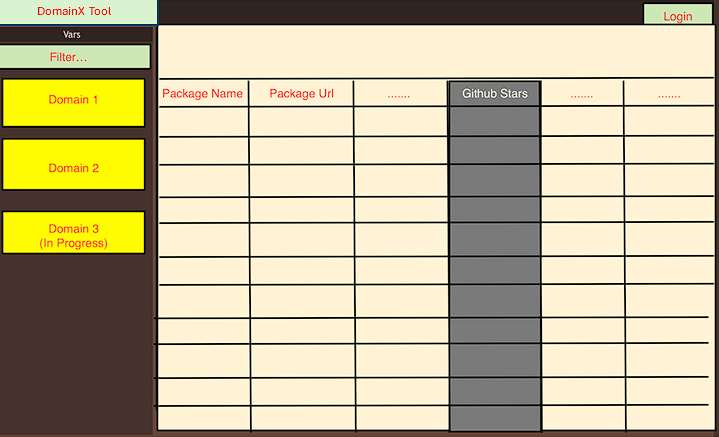
\includegraphics[totalheight=8cm]{images/DomainX-UI.png}
  \caption{DomainX UI, inspired by Octave Online}
  \label{fig:domainx_ui}
\end{figure}
\newpage{}
\section*{Appendix --- Reflection}

The purpose of reflection questions is to give you a chance to assess your own
learning and that of your group as a whole, and to find ways to improve in the
future. Reflection is an important part of the learning process.  Reflection is
also an essential component of a successful software development process.  

Reflections are most interesting and useful when they're honest, even if the
stories they tell are imperfect. You will be marked based on your depth of
thought and analysis, and not based on the content of the reflections
themselves. Thus, for full marks we encourage you to answer openly and honestly
and to avoid simply writing ``what you think the evaluator wants to hear.''

Please answer the following questions.  Some questions can be answered on the
team level, but where appropriate, each team member should write their own
response:


\begin{enumerate}
  \item What went well while writing this deliverable? 
  \item What pain points did you experience during this deliverable, and how did
  you resolve them?
  \item How many of your requirements were inspired by speaking to your
  client(s) or their proxies (e.g. your peers, stakeholders, potential users)?
  \item Which of the courses you have taken, or are currently taking, will help
  your team to be successful with your capstone project.
  \item What knowledge and skills will the team collectively need to acquire to
  successfully complete this capstone project?  Examples of possible knowledge
  to acquire include domain specific knowledge from the domain of your
  application, or software engineering knowledge, mechatronics knowledge or
  computer science knowledge.  Skills may be related to technology, or writing,
  or presentation, or team management, etc.  You should look to identify at
  least one item for each team member.
  \item For each of the knowledge areas and skills identified in the previous
  question, what are at least two approaches to acquiring the knowledge or
  mastering the skill?  Of the identified approaches, which will each team
  member pursue, and why did they make this choice?
\end{enumerate}


\end{document}